\documentclass{article}

% Language setting
% Replace `english' with e.g. `spanish' to change the document language
\usepackage[portuguese]{babel}

% Set page size and margins
% Replace `letterpaper' with`a4paper' for UK/EU standard size
\usepackage[a4paper,top=2cm,bottom=2cm,left=3cm,right=3cm,marginparwidth=1.75cm]{geometry}

% Useful packages
\usepackage{amsmath}
\usepackage{graphicx}
\usepackage[colorlinks=true, allcolors=blue]{hyperref}
\usepackage{float}
\usepackage{algorithm}
\usepackage{algpseudocode}

\graphicspath{{images/}}

\title{Projeto parcial \\
\large \textit{Closest string}}
\author{Lucas Emanuel Resck Domingues}

\begin{document}

    \maketitle
    
    \noindent \textbf{Tarefa 1} (1 ponto) Escolha um problema de otimização combinatória, apresente sua definição e apresente argumentos da sua NP-dificuldade (não é necessário fazer a redução ou a demonstração).

    \bigskip

    Vamos trabalhar o problema da \textbf{\textit{closest string}} (``string mais próxima'', em tradução livre). Dadas $n$ strings de tamanho $m$, $s_1, \cdots, s_n$, buscamos uma nova string $s$ de tamanho $m$ tal que $\text{d}(s_i, s) \le d$, para todo $i \in \{1, \cdots, n\}$, porém com $d$ sendo o menor valor possível. A função $\text{d}(\cdot, \cdot)$ é a distância de Hamming, \textit{i.e.}, o número de posições diferentes entre as duas strings. Vamos considerar, neste problema, um alfabeto fixo $\Sigma$.
Sendo assim, de forma um pouco mais abstrata, estamos buscando, no espaço métrico $\left(\Sigma^m, \text{d}\right)$ (espaço de Hamming), a menor bola fechada, com centro $s$ e raio $d$, que contém todas as $n$ strings $s_i$.

Vejamos um exemplo. Suponhamos que queremos encontrar a string mais próxima a ambas as strings \fbox{G}\fbox{A}\fbox{T}\fbox{O}, \fbox{G}\fbox{A}\fbox{M}\fbox{E} e \fbox{G}\fbox{A}\fbox{M}\fbox{O}. Então é óbvio que a solução será \fbox{G}\fbox{A}\fbox{?}\fbox{?}. Nossas opções para a terceira letra são T e M e para a quarta letra são O e E. Para cada combinação, temos o seguinte valor $d$ mínimo:
\begin{itemize}
    \item \fbox{G}\fbox{A}\fbox{T}\fbox{O} $\Rightarrow 2$
    \item \fbox{G}\fbox{A}\fbox{T}\fbox{E} $\Rightarrow 2$
    \item \fbox{G}\fbox{A}\fbox{M}\fbox{O} $\Rightarrow 1$
    \item \fbox{G}\fbox{A}\fbox{M}\fbox{E} $\Rightarrow 2$
\end{itemize}
Ou seja, nossa solução é \fbox{G}\fbox{A}\fbox{M}\fbox{O}.

O problema da \textit{closest string} é NP-difícil.
De forma intuitiva, vamos pensar em um problema mais simples, em que o alfabeto é $\Sigma = \{0, 1\}$. Então a string assume a forma $001 \cdots 01$, que, por acaso, é a representação do problema da mochila 0-1. No problema da mochila, você é incentivado a colocar um item pois ele tem valor positivo, mas é desincentivado pois tem peso positivo, e há restrição de peso. Você nunca sabe ``qual vale mais a pena'', se é deixar a mochila mais leve ou mais valiosa. Colocar um item, mesmo que leve e valioso, pode atrapalhar muito os outros itens, a ponto de deixar a mochila menos valiosa ao final. Isto é, não se sabe se é possível sacrificar um item para ter um ganho melhor com outros itens. O dilema é parecido nesse caso: você é incentivado a utilizar o caractere 0 pois isso vai se parecer com algumas \textit{strings}, porém é incentivado a utilizar o caractere 1 ao mesmo tempo, pois se parece com outras, e você não sabe qual vale mais a pena. Não se sabe se é possível sacrificar um caractere em uma posição para se ter um ganho melhor com outros caracteres em outras posições, e vice-versa.

Claro, essa intuição não prova nada. Uma demonstração da NP-dificuldade do problema é dada por \cite{frances1997covering}. A demonstração não é trivial, e não cabe neste trabalho.

    \newpage
    
    \noindent \textbf{Tarefa 2} (2,5 pontos) Proponha um algoritmo exato para a resolução deste     problema. Calcule sua complexidade.

    \bigskip

    O problema é NP-difícil, então não precisamos ter medo de algoritmos com complexidade exponencial. Vamos propor aqui um algoritmo de força bruta, que testa todas as soluções possíveis que faz sentido serem testadas.

Sejam $s_1, \cdots, s_n$ as $n$ strings de tamanho $m$. Então, para cada posição $i$, a string $s$ pode assumir algum dos valores $S_i = \left\{s_1[i], \cdots, s_n[i]\right\}$. Nosso algoritmo será aquele que testa cada uma das combinações possíveis com $S_1$ para a posição 1 de $s$, $S_2$ para a posição 2 de $s$, $\cdots$, $S_m$ para a posição $m$ de $s$, e no final escolhe a melhor das soluções. Na verdade, é mais prático manter uma variável indicando a melhor das soluções durante a iteração e atualizando-a quando necessário.

Para uma determinada posição $i$, $S_i = \{s_1[i], \cdots, s_n[i]\}$ é todo o alfabeto $\Sigma$, no pior caso. Logo, como são $m$ posições, o número de combinações possíveis para $s$ é $O(|\Sigma|^m)$.

Para cada combinação de $s$, são necessários $n$ cálculos de distância de Hamming com as outras strings $s_i$, que, cada um, toma tempo $O(m)$.
Depois de calcular todos os $\text{d}(s, s_i)$, precisamos encontrar o maior desses valores, o que pode ser feito em tempo linear.
Ou seja, esse algoritmo tem complexidade $O((mn+n)|\Sigma|^m) = O(mn|\Sigma|^m)$.

    \newpage
    
    \noindent \textbf{Tarefa 3} (3 pontos) Proponha e implemente um algoritmo baseado em árvores
    ou por aproximação. Apresente argumentos para sua corretude e/ou aproximação e calcule sua complexidade.

    \bigskip

    No que diz respeito a algoritmos de aproximação, \cite{li2002closest} propôs, e demonstrou, uma aproximação em tempo polinomial com razão de aproximação $1 + \epsilon$ para o problema da \textit{closest string}, como descrito na Tarefa 1.
A implementação do algoritmo não é trivial e acredito que esteja um pouco além do que é requerido por este trabalho. Além disso, não existe uma implementação desse algoritmo acessível, então decidi por não me estender muito nesse resultado.

Vamor propor e implementar, nesta tarefa, um algoritmo no estilo \textit{branch and bound}, que nos permita explorar todas as soluções, porém ignorar aquelas em que temos certeza que não são boas o suficiente. Imagine que o Algoritmo \ref{alg:exact} funcione a partir de ramificações. Ou seja, o primeiro nó da árvore é vazio e possui como filhos todas as possibilidades para a primeira letra; escolhido um filho, seus filhos possuem todas as possibilidades para a segunda letra; e assim por diante, como na \autoref{fig:tree}. Esse é o \textit{branch}.

\begin{figure}[H]
    \centering
    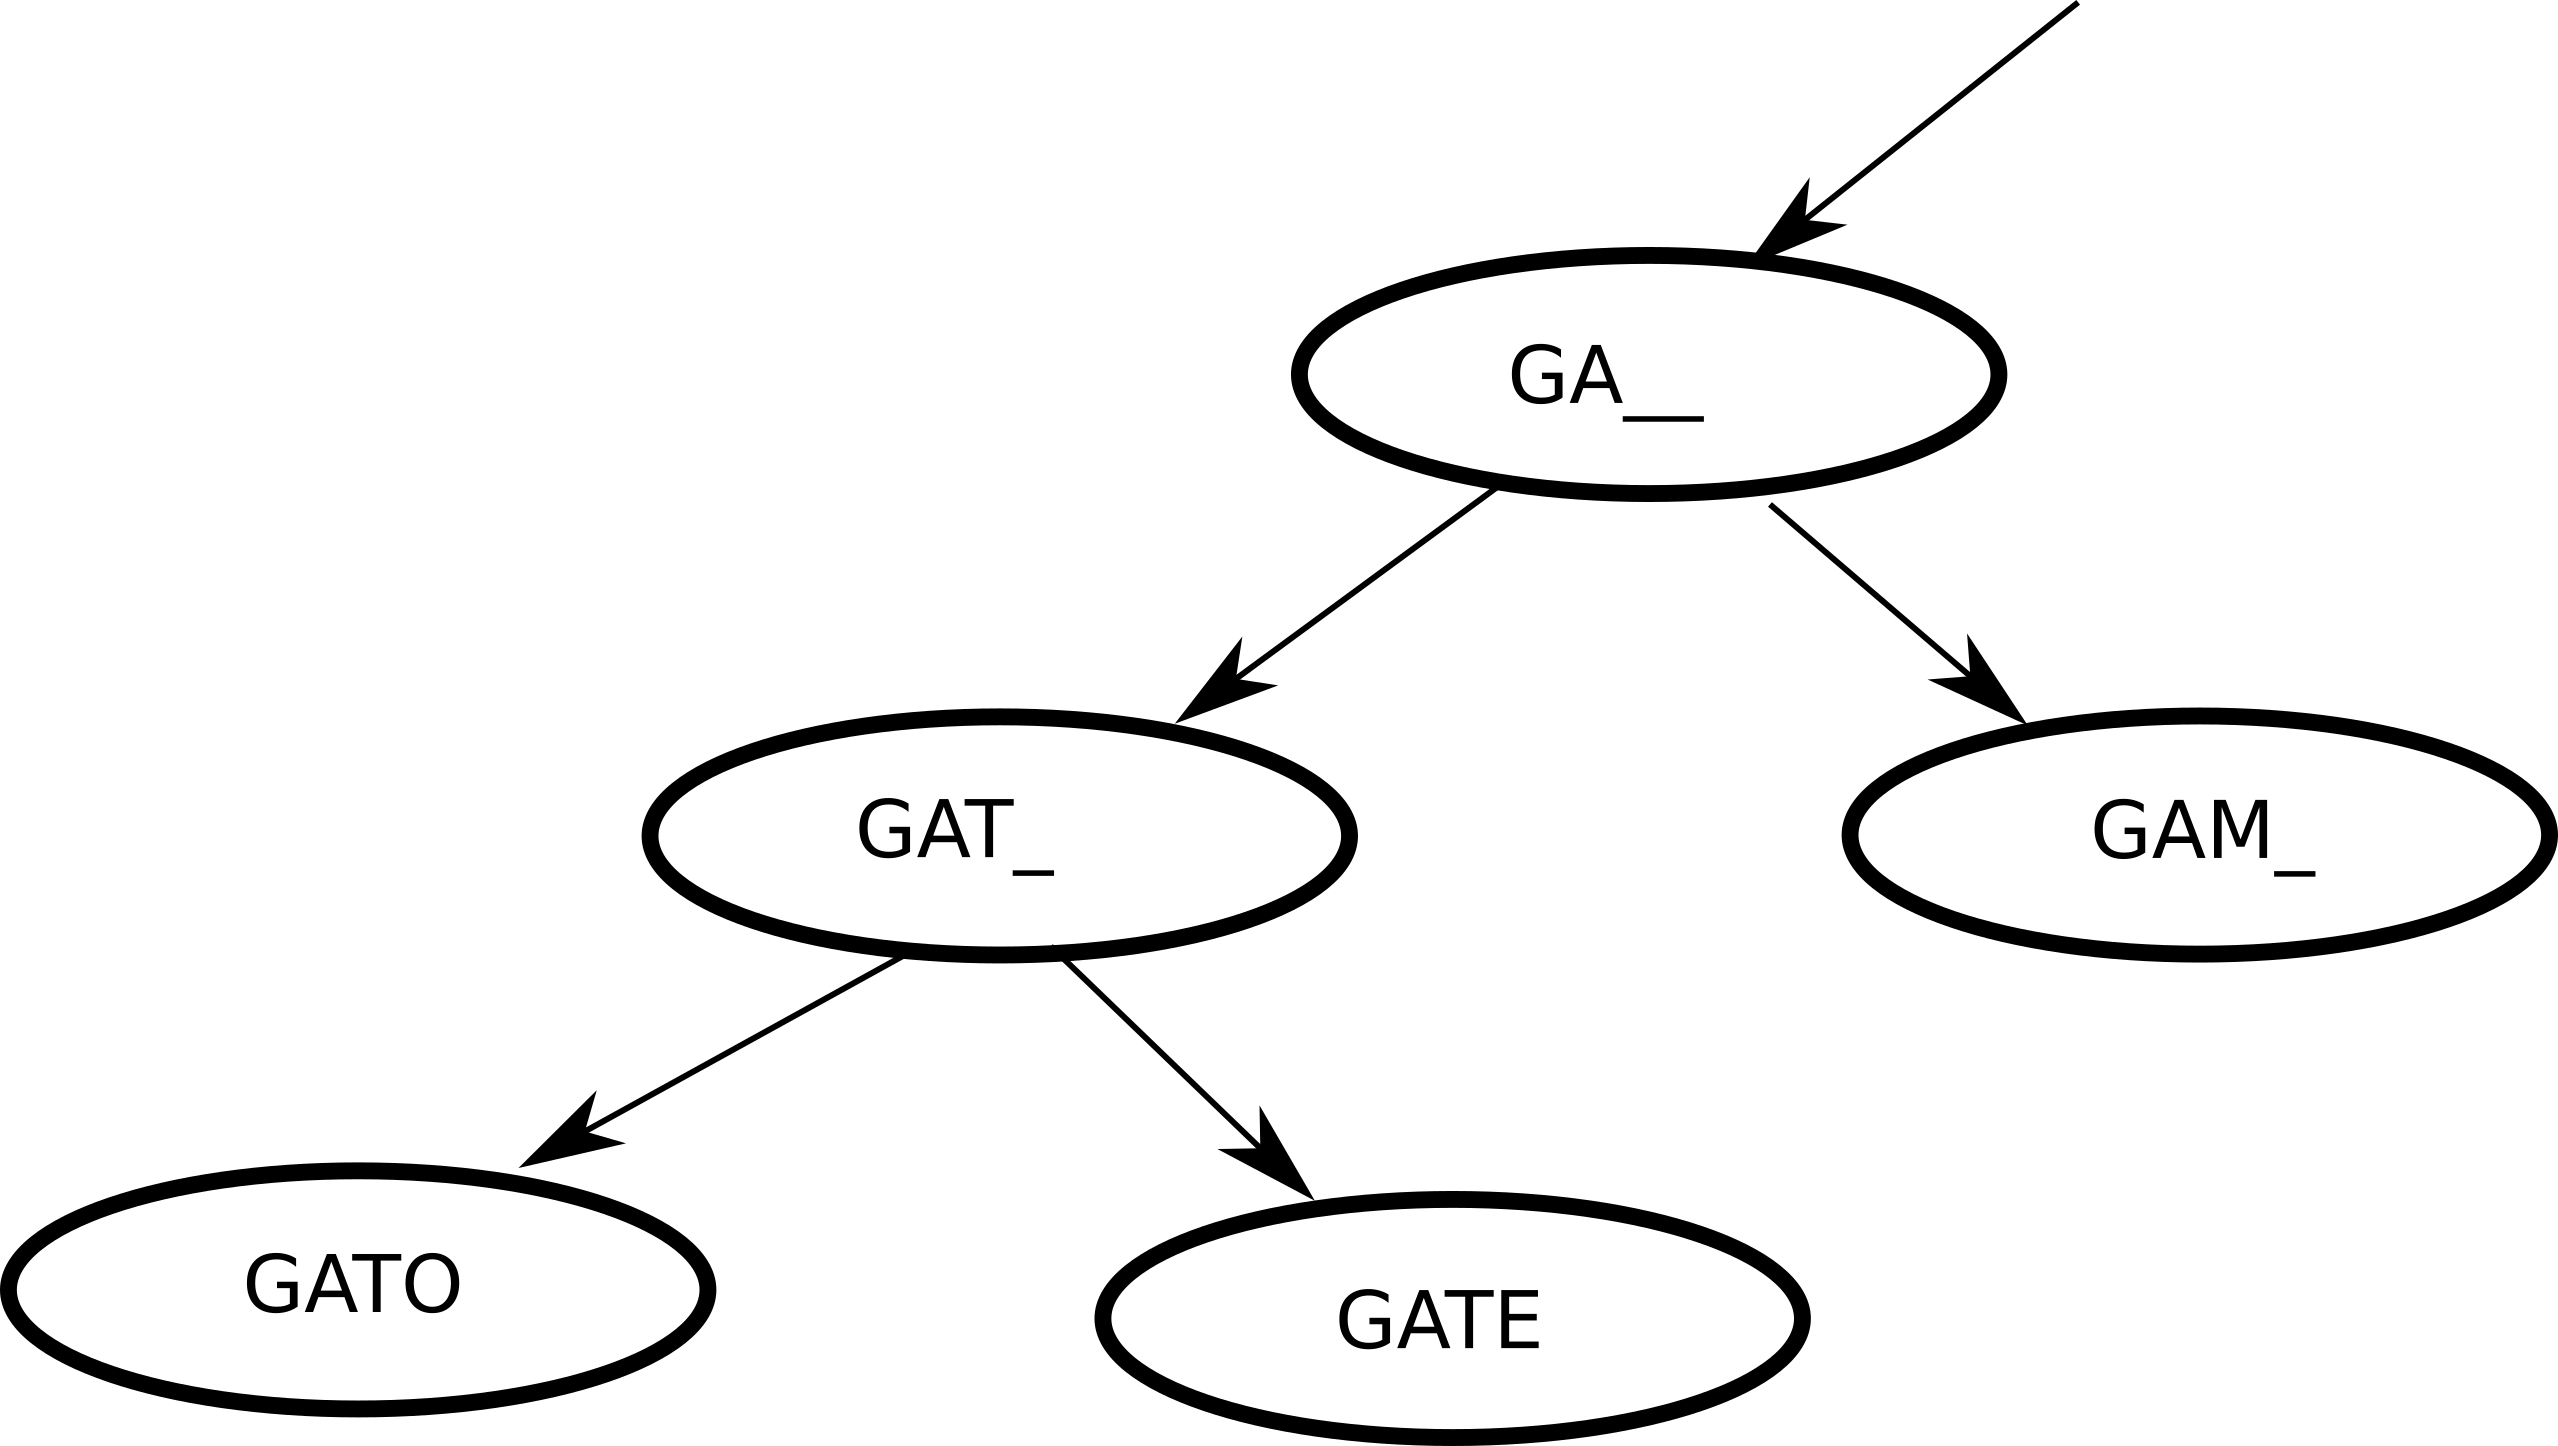
\includegraphics[width=0.6\linewidth]{tree.png}
    \caption{Exemplo de árvore.}
    \label{fig:tree}
\end{figure}

Para saber se é válido explorar uma subárvore, isto é, quando realizar o \textit{bound}, vamos utilizar um \textit{lower bound} para o menor custo $d$ em uma subárvore. Note que, em um nó com as $i$ primeiras letras definidas, temos o custo dessas $i$ primeiras letras já calculado; precisamos nos preocupar apenas com as $m-i$ letras restantes, isto é, $s[i+1:m]$. Note que, se quisermos minimizar a soma das distâncias de Hamming de $s[i+1:m]$ às strings $s_1[i+1:m], \cdots, s_n[i+1:m]$, basta que tomemos, em cada posição, aquela letra mais comum para aquela posição. Seja essa a string $s^\ast$. Ora, se $d_{OPT}$ é custo mínimo ótimo para as strings $s_1[i+1:m], \cdots, s_n[i+1:m]$, com centro $s^{\ast\ast}$, então vale que $\text{d}(s^{\ast\ast}, s_i[i+1:m]) \le d_{OPT}$ para todo $j$, de forma que
\[\sum_j \text{d}(s^{\ast\ast}, s_j[i+1:m]) \le n d_{OPT},\]
e, finalmente,
\[\frac{\sum_j \text{d}(s^{\ast}, s_j[i+1:m])}{n} \le \frac{\sum_j \text{d}(s^{\ast\ast}, s_j[i+1:m])}{n} \le d_{OPT},\]
sendo a primeira desigualdade justificada pelo fato de que $s^\ast$ minimiza a soma das distâncias de Hamming.
Ou seja, a soma das distâncias de Hamming a $s^\ast$ (a string de $i+1$ a $m$ que toma as letras mais comuns) sobre $n$ é um lower bound para o custo ótimo de uma subárvore, ignorando as $i$ primeiras posições. Isso, somado ao custo das $i$ primeiras posições, nos dá um \textit{lower bound} para o custo ótimo de uma subárvore. Sendo assim, não precisamos explorá-la caso já tenhamos uma solução melhor.
O Algoritmo \ref{alg:tree} descreve um pseudocódigo para essa solução.

\begin{algorithm}[H]
    \caption{Algoritmo \textit{branch and bound} para o problema da \textit{closest string}.}
    \label{alg:tree}
    \begin{algorithmic}
        \Require Strings $s_1, \cdots, s_n$ de tamanho $m$
        \State Cria os conjuntos $S_i = \left\{s_1[i], \cdots, s_n[i]\right\}$, para cada $i$
        \State Inicializa uma solução qualquer $s_0$
        \State Calcula o valor $d_0$ da solução $s_0$
        \State $s \gets$ empty string
        \State $\textsc{branch}(s)$        
        \State \Return $s_0, d_0$
        \State
        \Procedure{branch}{$s$}
            \State $i = \text{length}(s)$
            \If{$i=m$}
                \State $d \gets$ custo de $s$
                \If{$d < d_0$}
                    \State $s_0 \gets s$
                    \State $d_0 \gets d$
                \EndIf
                \State \Return
            \EndIf
            \State $l \gets$ \textit{lower bound} para o custo mínimo de $s$ \Comment{Aqui usamos o que foi descrito na solução.}
            \If{$l > d_0$}
                \State \Return
            \EndIf
            \For{char $\in S_i$}
                \State $\textsc{branch}(s + \text{char})$ \Comment{Estamos adicionando char à string $s$.}
            \EndFor
        \EndProcedure
    \end{algorithmic}
\end{algorithm}

A implementação do Algoritmo \ref{alg:tree} for realizada em Python, podendo ser conferida \href{https://github.com/lucasresck/data-structures-algorithms/blob/main/intractable_problems/scripts/closest_string_tree.py}{neste link}. Por exemplo, se pedirmos ao programa qual a \textit{closest string} para 
\[\overset{\underbrace{\text{\fbox{G}\fbox{A}\fbox{T}\fbox{O}}\cdots\text{\fbox{G}\fbox{A}\fbox{T}\fbox{O}}}}{\text{8 vezes}}\]
\[\overset{\underbrace{\text{\fbox{G}\fbox{A}\fbox{M}\fbox{E}}\cdots\text{\fbox{G}\fbox{A}\fbox{M}\fbox{E}}}}{\text{8 vezes}}\]
\[\overset{\underbrace{\text{\fbox{G}\fbox{A}\fbox{M}\fbox{O}}\cdots\text{\fbox{G}\fbox{A}\fbox{M}\fbox{O}}}}{\text{8 vezes}}\]
obtemos 
\[\overset{\underbrace{\text{\fbox{G}\fbox{A}\fbox{M}\fbox{O}}\cdots\text{\fbox{G}\fbox{A}\fbox{M}\fbox{O}}}}{\text{8 vezes}}\] em 28779 iterações. Um ponto importante é que, sem o \textit{bound}, esse número se torna 174761, significantemente maior.

A corretude do algoritmo é direta, pois é herdada do algoritmo da Tarefa 2 (que é exato) juntamente com a corretude do \textit{bound}, como discutido anteriormente. Porém, esse processo de \textit{bound} não garante que um número significativo de casos será eliminado: ainda, no pior caso, poderíamos passar por todos os nós.
Note que nosso Algoritmo \ref{alg:tree} é essencialmente o Algoritmo \ref{alg:exact}, porém no formato de árvore (com recursões), além do fato de que são calculados os lower bounds. O cálculo do lower bound tem complexidade $O(nm + m)$\footnote{Para perceber isso, veja que a primeira parcela se refere ao custo atual até a posição $i$, enquanto a segunda parcela se refere ao lower bound a partir da posição $i+1$. Esse custo é linear, pois é possível ter os ``custos de cada posição'' previamente calculados. Para mais detalhes, por favor, conferir a implementação.}.
Como a quantidade de nós é $O(|\Sigma|^m)$, isso faz com que a complexidade do algoritmo continue a mesma da Tarefa 2: $O(mn|\Sigma|^m)$.


    \newpage

    \bibliographystyle{alpha}
    \bibliography{references}

\end{document}